\chapter{Test Cases} \label{6Testing}

This chapter details the reasoning and design of the test cases used in this thesis. To provide a common platform for comparing \gls{ble} and 802.15.4, Contiki was ported to a platform supporting \gls{ble} as described in chapter \ref{5bleContiki}. This chapter starts off with section \ref{6Metrics} explaining all the metrics measured in the experiments performed. Section \ref{6TestPlatforms} follows by explaining the test platforms and tools used. Section \ref{6HTdesign} and \ref{6RRdesign} explains the two test suite designed to measure the metrics defined.

% % % % % % % % % % % % SECTION % % % % % % % % % % % % 

\section{Performance Metrics Definition} \label{6Metrics}
The aim of this thesis is to compare the key characteristics of the link layer of \gls{ble}  and 802.15.4. Note that as explained in section \ref{Overview15.4}, 802.15.4 here means the physical layer of 802.15.4 standard. The 802.15.4 standard \gls{mac} layer is not used, rather Null-RDC and ContikiMAC was used, both with \gls{csma} layer. The scenario looked into in this thesis is of the case where there is communication between two device, one constrained in terms of power and the other not. This is typical of \emph{appcessories}, where one device is a powerful mobile device and the other is a battery operated single purpose device.
In this section the four key performance metrics measured for both the wireless protocols are defined in the context of this thesis.

\paragraph{Data Rate}
Data rate at the link layer is defined as the maximum amount of data transmitted per second for a protocol with packets containing the maximum allowed payload for the link layer. The data rate is expressed as both kilobits per second and packets per second.

\paragraph{Latency}  \label{6para:latency}
\begin{wrapfigure}{r}{0.52\textwidth}
	\vspace{-10pt}
	\centering
	\capstart
	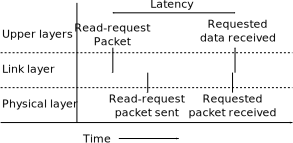
\includegraphics{LatencyDef}
	\caption{Illustration of latency measurement}
	\vspace{-10pt}
	\label{fig:LatencyDef}
\end{wrapfigure}
In this test the aim is to measure the effect of the link layer architecture and configuration on the latency observed by an layer on top when requesting data from another node. Latency is defined as the time from which the layer(s) above the link layer provides it the packet which asks for data from another node to the time the data from the other node is received. This is better understood by a generic illustration in figure \ref{fig:LatencyDef}.

\paragraph{Reliability}
Two criteria was used for measuring reliability when two nodes are communicating. \gls{prr} is defined as the ratio of the number of packets successfully received to the number of packets sent, both by the link layer. \gls{pdr} is defined as the ratio of the number of packets delivered to the number of packets sent, by the layer above the link layer in both the sender and receiver. While \gls{prr} measures the reliability of transfer of a single transfer of a packet, \gls{pdr} measures the reliability of the link layer to communicate a packet as seen by the layer above it.

\paragraph{Energy Consumption}
The energy consumption in this project is indirectly measured as the \acrfull{rdc}, which is the ratio of the time for which the radio is switched on to the total time of the experiment. Measuring the energy consumption as \gls{rdc} for different scenarios will be more useful to developers as this information will change little across platforms for the same protocol, whereas the actual energy consumed is reducing with every new platform introduced in the market, as seen in this presentation\cite{Bernegger2014}. The processor time utilized by the protocol stack is not considered as this information could not be extracted from the SoftDevice \glspl{api} and also because of the different processor types in the two platforms (32-bit vs 16 bit). 

% % % % % % % % % % % % SECTION % % % % % % % % % % % % 

\section{Test Setup} \label{6TestPlatforms}

\subsection{\texorpdfstring{\gls{ble}}{BLE} Platform}
The platform used for \gls{ble} is PCA10000, which is described in section \ref{5nrfPCA}. Since \gls{ble}  is has an asymmetric architecture, a master device is required to communicate with a slave device. In all the tests the slave device is a PCA10000 board running on Contiki and peripheral \gls{ble}  stack provided by the SoftDevice \emph{S110} version 6.0.0. Depending on the test, the master device varied between either a PCA10000 board or an Android device. When a PCA10000 was used as master device, it ran on bare-metal code with central \gls{ble} stack provided by the SoftDevice \emph{S120} version 1.0.0. This choice of use of Contiki for slave and bare-metal code for master is consistent with the assumption that the master is unconstrained and slave is not. The transmission power was 0 dBm for all the tests using PCA10000. Nexus 7 and Nexus 4, both at Android version 4.4.4 were the Android devices used for performing certain tests.

Communication was done at the Generic Attribute (GATT) layer because the binary from Nordic Semiconductor used in this project does not provide APIs to access the lower layers in both peripheral and central devices, hence evaluation at the link layer was done indirectly based on the inferences from the collected data. The default transmission power of 0 dBm was used. The radio state change notification event in the SoftDevice was enabled. This allowed logging of a timer to measure the energy consumption in terms of \gls{rdc}.

\subsection{802.15.4 Platform}

\begin{figure}[h]
    \centering
    \includegraphics[width=\textwidth]{TmoteSky}
	\caption{TmoteSky platform}
    \label{fig:TmoteSky}
\end{figure}

Tmote-Sky platform, which is widely used and supports all the features of Contiki was used as the platform to test 802.15.4 performance. Shown in figure \ref{fig:TmoteSky}, Tmote-Sky is based on MSP430-F1611 \gls{mcu} and  CC2420 2.4 GHz transceiver. It has a USB to serial converter on board to allow the MSP430 \gls{mcu} to communicate with the serial port of a computer. It has additional sensors, buttons and memory which are not used in this project. The transmission power was unchanged from the default value of 0 dBm. The `energest' module of Contiki was used to log the radio on and total time to calculate the energy consumption in terms of \gls{rdc}. 

\subsection{WiFi Interference}
In some of the tests described in the following sections, WiFi interference needed to be created to test the reliability of the wireless protocols with external interference. A open-source tool called \texttt{iperf} was used for creating this interference by sending \gls{udp} packets to the IP address of a router. The computer and router used are ThinkPad T420 and Netgear N300 router respectively, both supporting WiFi 802.11b/g/n standard. The aim of the interference pattern is to simulate streaming of large amount of data over WiFi. This was achieved by this command:

\texttt{sudo iperf -c 192.168.1.1 -u -P 1 -i 1 -p 5001 -f M -b 54.0M -t 64 -T 1}

Where `-c 192.168.1.1' specifies that the packets are sent to the IP address specified (router's IP), `-u' to use \gls{udp} packets, `-P 1' specifies one client thread to run, `-i 1' specifies the bandwidth reporting interval as one second, `-p 5001' specifies the server port to connect to as 5001, `-f M' specifies the reporting format as MegaByte per second, `-b 54.0M' specifies the data rate to be used as 54 Megabit per second, `-t 64' specifies the transmission to happen for 64 second and `-T 1' specifies that only one hop is allowed to reach destination. Although the data rate was specified as 54 Mbps i.e. 6.75 MBps, the actual data rate of transmission reported was around 3 MBps. 

\begin{figure}[h]
	\begin{subfigure}[b]{1\textwidth}
		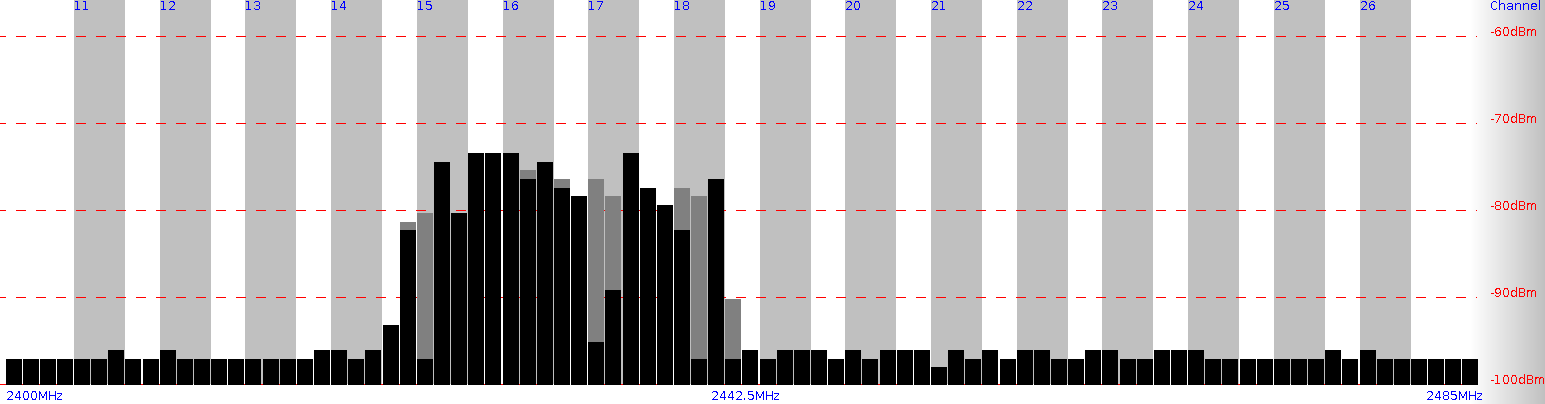
\includegraphics[width=\textwidth]{Intf}
		\caption{Environment while running iperf tool to create interference}
		\vspace{10pt}
		\label{fig:Intf}
	\end{subfigure}

	\begin{subfigure}[b]{1\textwidth}
		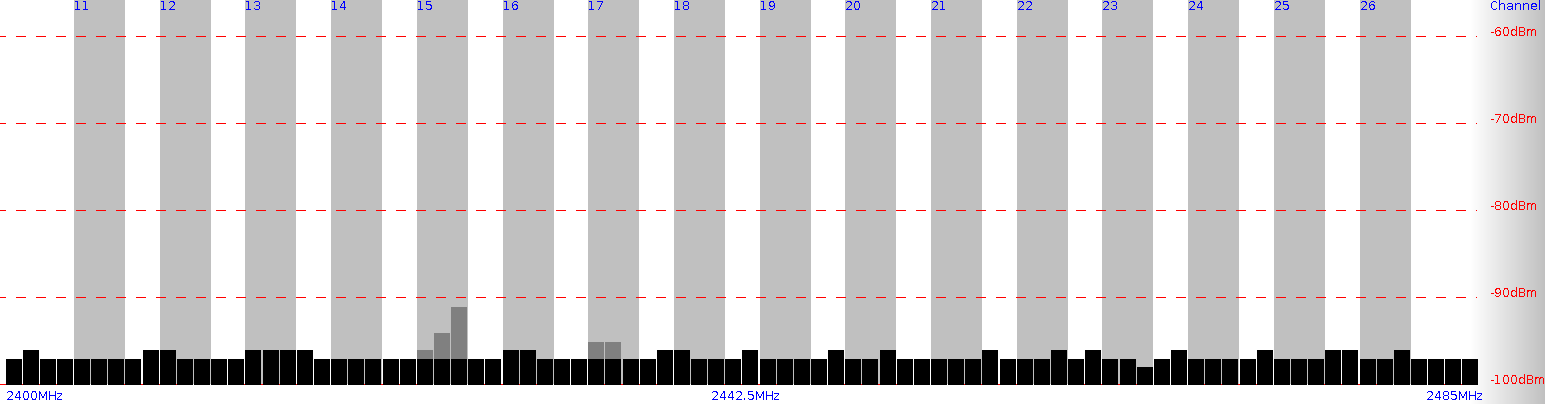
\includegraphics[width=\textwidth]{NoIntf}
		\caption{Environment without creating interference}
		\label{fig:NoIntf}
	\end{subfigure}
	\caption{2.4 GHz environment captured by rssi-scanner}
	\vspace{-10pt}
\end{figure}


To verify that the interference was created and to know which frequency range was occupied, the `rssi-scanner' project was used\footnote{Available at: http://sourceforge.net/p/contikiprojects/code/HEAD/tree/sics.se/rssi-scanner/}. This project is based on Tmote-Sky platform running on Contiki. The screen-shot of rssi-scanner shows a snapshot of the environment where the test were conducted for the cases of with and without interference in figure \ref{fig:Intf} and \ref{fig:NoIntf} respectively, where y-axis shows the signal strength measured and x-axis is the frequency of the measurement.


% % % % % % % % % % % % SECTION % % % % % % % % % % % % 

\section{\texorpdfstring{\acrfull{ht}}{High-Throughput} Test Design} \label{6HTdesign}
\gls{ht} test aims to measure the maximum possible data rate of \gls{ble} and 802.15.4 at the LL with and without WiFi interference. For both protocols, the link layer contains the maximum payload allowed. Each run of the test will last for one minute to collect enough data to calculate the mean data rate. In each of the tests, the amount of time the radio is switched on (\gls{rdc}), either transmitting or receiving, is logged to measure the energy consumption. The metrics measured in this test are data rate, reliability and energy consumption. The two nodes were kept 1 m apart and in case of environment with interference, the router to which the \gls{udp} packets were sent over WiFi was about 2.5 m from these nodes. In the cases where an Android device is not involved, they were conducted for 10 times and the median value of the 10 was used. The test with an Android device could not be automated, so the test was conducted once.

\begin{figure}[h]
\def\svgwidth{\columnwidth}
\input{./Images/layout.pdf_tex}
%
\includegraphics[width=\textwidth]{layout}
\caption{Test setup for \gls{ht} test cases}
\label{fig:layout}
\end{figure}

\begin{wrapfigure}{r}{0.53\textwidth}
	\vspace{-20pt}
	\centering
	\capstart
	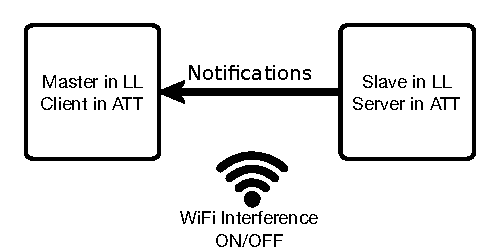
\includegraphics{DataRateSetup.pdf}
	\caption{Setup to measure data rate with \gls{ble}}
    \label{fig:DataRateSetup}
%   	\vspace{-15pt}
\end{wrapfigure}

\paragraph{\texorpdfstring{\gls{ble}}{BLE}} As shown in figure \ref{fig:DataRateSetup}, the data rate is measured by sending data from the server to the client using \emph{Notifications}, which are packets which are not acknowledged in the \gls{att} layer. Since the link layer is not accessible with the SoftDevice used, a 20 byte payload was sent at the \gls{gatt} layer as notification so that 27 byte data for the link layer's playload is achieved. The data rate is measured at the receiver i.e the Master device. 

The number of packets sent and received at the \gls{att} layer in the two nodes are logged to calculate the \gls{pdr}. Also by logging the number of times the radio was switched on, the number of packets actually transmitted can be inferred, by which the \gls{prr} can be calculated.

\gls{ble}  specification tells that a master device must change the channel map of a connection according the 2.4 GHz environment so as to not face any interference. This is the \emph{adaptive} part of \gls{afh}, which requires the master device to have information about the activity in the frequency spectrum used by \gls{ble} . S120 SoftDevice used for the central \gls{ble}  stack by default uses the complete channel map and has an option for configuring it manually, but the channel map does not change automatically based on external interference. So in the tests without WiFi interference, the channel map consisted of all the channels. When WiFi interference was introduced, one test had the complete channel map and another had a \emph{WiFi free} map of channels (0 to 6) and (20 to 36), which is 2404 to 2416 MHz and 2446 to 2478 MHz. This map was based on the interference noticed in figure \ref{fig:Intf}.

\paragraph{802.15.4} In case of 802.15.4, Null-RDC layer was modified to send packets with maximum payload size as soon as possible. One node is configured as transmitter and the other as receiver, with the data rate measured at the receiver. A payload of 110 byte was necessary for the link layer to achieve the maximum 127 byte packet size.

Three tests were designed to measure the data rate achievable with 802.15.4. In the first test without WiFi interference, channel 26 (2480 MHz) of 802.15.4 was used. In the second test with WiFi interference, channel 15 (2425 MHz) of 802.15.4 was used. In the third test, the \gls{cca} was disabled, so that the transmitting node ignores the external environment.

The various test cases conducted in the \gls{ht} test suite are 
\vspace{-5 pt}
\begin{multicols}{2}
\begin{itemize} \itemsep1pt \parskip0pt \parsep0pt
\item sky\_sky\_N\_!CCA
\item sky\_sky\_Y\_26
\item sky\_sky\_Y\_15
\item nrf\_nrf\_N\_all
\item nrf\_nrf\_Y\_all
\item nrf\_nrf\_Y\_!Wifi
\item nrf\_N4\_N
\item nrf\_N7\_N
\end{itemize}
\end{multicols}


The legend of the naming of the test cases is

\texttt{\{source\}\_\{destination\}\_\{presence of WiFi interference(Y/N)\}\_\{other conditions\}}

Where,
sky = Tmote-Sky;	nrf = nrf51822;	N4 = Nexus4; 		N7 = Nexus7;
!CCA = CCA disabled; 26,15 = channel used; all = All 40 \gls{ble}  channels;	!WiFi = WiFi free channels in \gls{ble} 


% % % % % % % % % % % % SECTION % % % % % % % % % % % % 
\section{\texorpdfstring{\acrfull{rr}}{Request-Response} Test Design} \label{6RRdesign}
The \gls{rr} test aims to determine the latency for reading data from another node as explained in the latency paragraph in section \ref{6Metrics}. In all the tests the nodes were kept at a distance less than 10 cm from one another, since the tests we aimed to reflect an error-free environment. In this tests also the time the radio is switched on is logged in both the nodes to calculate \gls{rdc} to interpret the energy consumption. The idea is to find the relation between energy consumption and latency based on different link layer configurations. Thus, the metrics evaluated in this test are latency and energy consumption.

\begin{figure}[h]
\centering
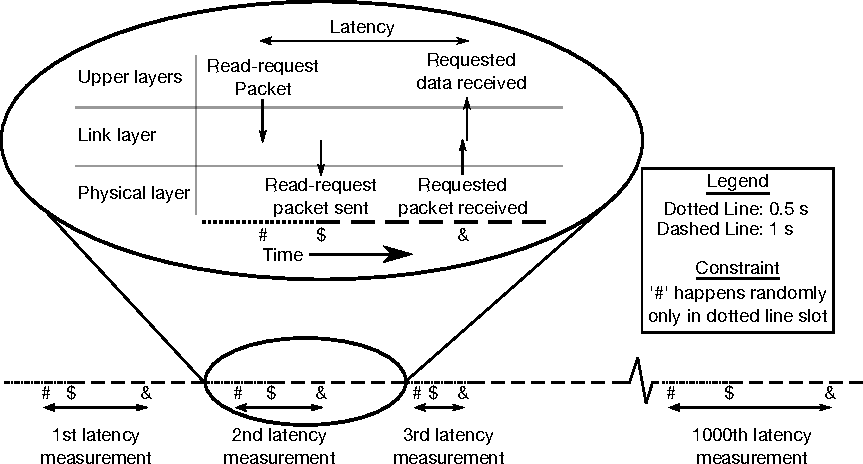
\includegraphics{RRTest}
\caption{Illustration of the RR Test operation}
\label{fig:RRTest}
\end{figure}

In all the tests performed, there is a \emph{requester} node and a \emph{responder} node. As explained in the latency paragraph in section \ref{6Metrics}, the latency is measured in the requester node. It is defined as the time from when the requester node \emph{needs} data from a responder to the time the responder node sends the requested data. This is better illustrated in the design of the test for both the protocols in figure \ref{fig:RRTest}. This figure shows the perspective of the requester node where the latency measurement takes place. A latency measurement is done in every 1.5 second period, repeated thousand times. The link layer is sent a `read-request' packet from its upper layer after a random time in the first 0.5 second slot of this 1.5 second period, represented by `\#' in figure \ref{fig:RRTest}. This randomization of the issuing of the read request (`\#' event) ensures that if there is any periodic communication between the nodes, the thousand measurements of latency will provide the range of values that can expected with a particular scenario along with the power consumption. In figure \ref{fig:RRTest}, the latency measurement is the difference of the time between the `\&' and `\#' events.


\paragraph{\texorpdfstring{\gls{ble}}{BLE}}
In case of \gls{ble} , the use case for the latency test is a central device which is master at link layer and client at \gls{att} layer needs to get data from a peripheral device which is slave at link layer and server at \gls{att}. This can be achieved with two configurations as shown in figure \ref{fig:RR_Read} and \ref{fig:RR_Indicate}. In both cases it is the \gls{att} client which gets the data from the server. In the first case, the client asks for the data from the server, which responds with data. So, the requester node is the master node (Client) and the responder is the slave node (Server). The latency measurement happens at the requester i.e. the master node. In the second case, the server sends the data in an `indication' packet, which is acknowledged by the client. In this case since it is the slave node that is getting the response from the master, the latency measurement happens in the slave node which is the requester here.

\begin{figure}[h]
	\vspace{10 pt}
	\begin{subfigure}[t]{0.49\linewidth}
		\centering
		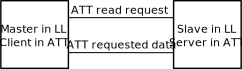
\includegraphics{RR_Read}
		\subcaption{Read-response test case}
		\label{fig:RR_Read}
	\end{subfigure}
	\begin{subfigure}[t]{0.49\linewidth}
		\centering
		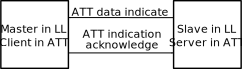
\includegraphics{RR_Indicate}
		\subcaption{Indicate-acknowledge test case}
		\label{fig:RR_Indicate}
	\end{subfigure}
	\caption{Test modes for measuring latency using \gls{ble}}
\end{figure}

\begin{table}[h]
\begin{center}
%\vspace{5pt}
\setlength{\extrarowheight}{1.5pt}
    \begin{tabular}{|l|l|l|l|}
\hline Test Case & Connection Interval & Slave Latency & Test Mode \\
\hline 7.5\_0\_r & 7.5 ms              & 0             & Read      \\
\hline 7.5\_0\_i & 7.5 ms              & 0             & Indicate  \\
\hline 7.5\_65\_r& 7.5 ms              & 65            & Read      \\
\hline 7.5\_65\_i& 7.5 ms              & 65            & Indicate  \\
\hline 125\_0\_r & 125 ms              & 0             & Read      \\
\hline 125\_0\_i & 125 ms              & 0             & Indicate  \\
\hline 125\_3\_r & 125 ms              & 3             & Read      \\
\hline 125\_3\_i & 125 ms              & 3             & Indicate  \\
\hline
    \end{tabular}
    \caption{List of \gls{rr} test cases using \gls{ble}}
    \vspace{-20pt}
    \label{tbl:RRTestsBLE}
    \end{center}
\end{table}


In all the tests, the complete payload of 20 bytes for the \gls{att} layer was used, which corresponds to 27 byte in the link layer. Two connection intervals of 7.5 ms and 125 ms were used for the tests. For each 'connection interval', tests were conducted with two different `slave latency' parameter. The table \ref{tbl:RRTestsBLE} shows these values and the configuration for all the test cases in \gls{rr} test using \gls{ble}. The intent here is to find the effect of the link layer configuration on the latency. By using different slave latency values, the energy consumption of the asymmetric connecting devices can be evaluated. The value of these configurations is decided such that the worst case theoretical latency in a error free environment is less than one second. This is the reason for choosing the `supervision timeout' of 1.5 s.

\paragraph{802.15.4}
In the case of 802.15.4, one node is configured to send unicast messages and another is configured to receive these and send a response. The latency was measured using both ContikiMAC and Null-RDC. ContikiMAC uses the default 125 ms wake up interval for the receiver. For payload size is same as in the test cases with \gls{ble}  for comparing the latency for the same payload. The \gls{ble} test cases are designed such that the 7.5 \si{\milli\second} connection interval tests can compare with Null-RDC test of 802.15.4 while the 125 \si{\milli\second} connection interval tests can compare with the ContikiMAC test of 802.15.4.

The sending of the unicast packet and getting its response followed the same thousand iterations of 1.5 s intervals containing a 0.5 s period where the packet was randomly requested to be sent. The latency measurement happens as illustrated by figure \ref{fig:LatencyDef} used to define the term latency in section \ref{6Metrics}.